\newpage
    
\chapter{Partie II : Matériel et Expérimentation}

La mise en œuvre pratique du docking autonome nécessite une intégration matérielle rigoureuse et une validation progressive. Cette partie décrit la plateforme robotique, le capteur principal, ainsi que les deux phases expérimentales menées pour valider nos algorithmes.

\section{Plateforme Robotique : BlueROV Heavy}

Dans cette section, nous présentons le matériel utilisé pour la réalisation de notre projet de docking via notre BlueROV.

Nous présenterons ses spécificités techniques dans les grandes lignes.


\subsection{Matériel}

\begin{figure}[h!]
    \centering
    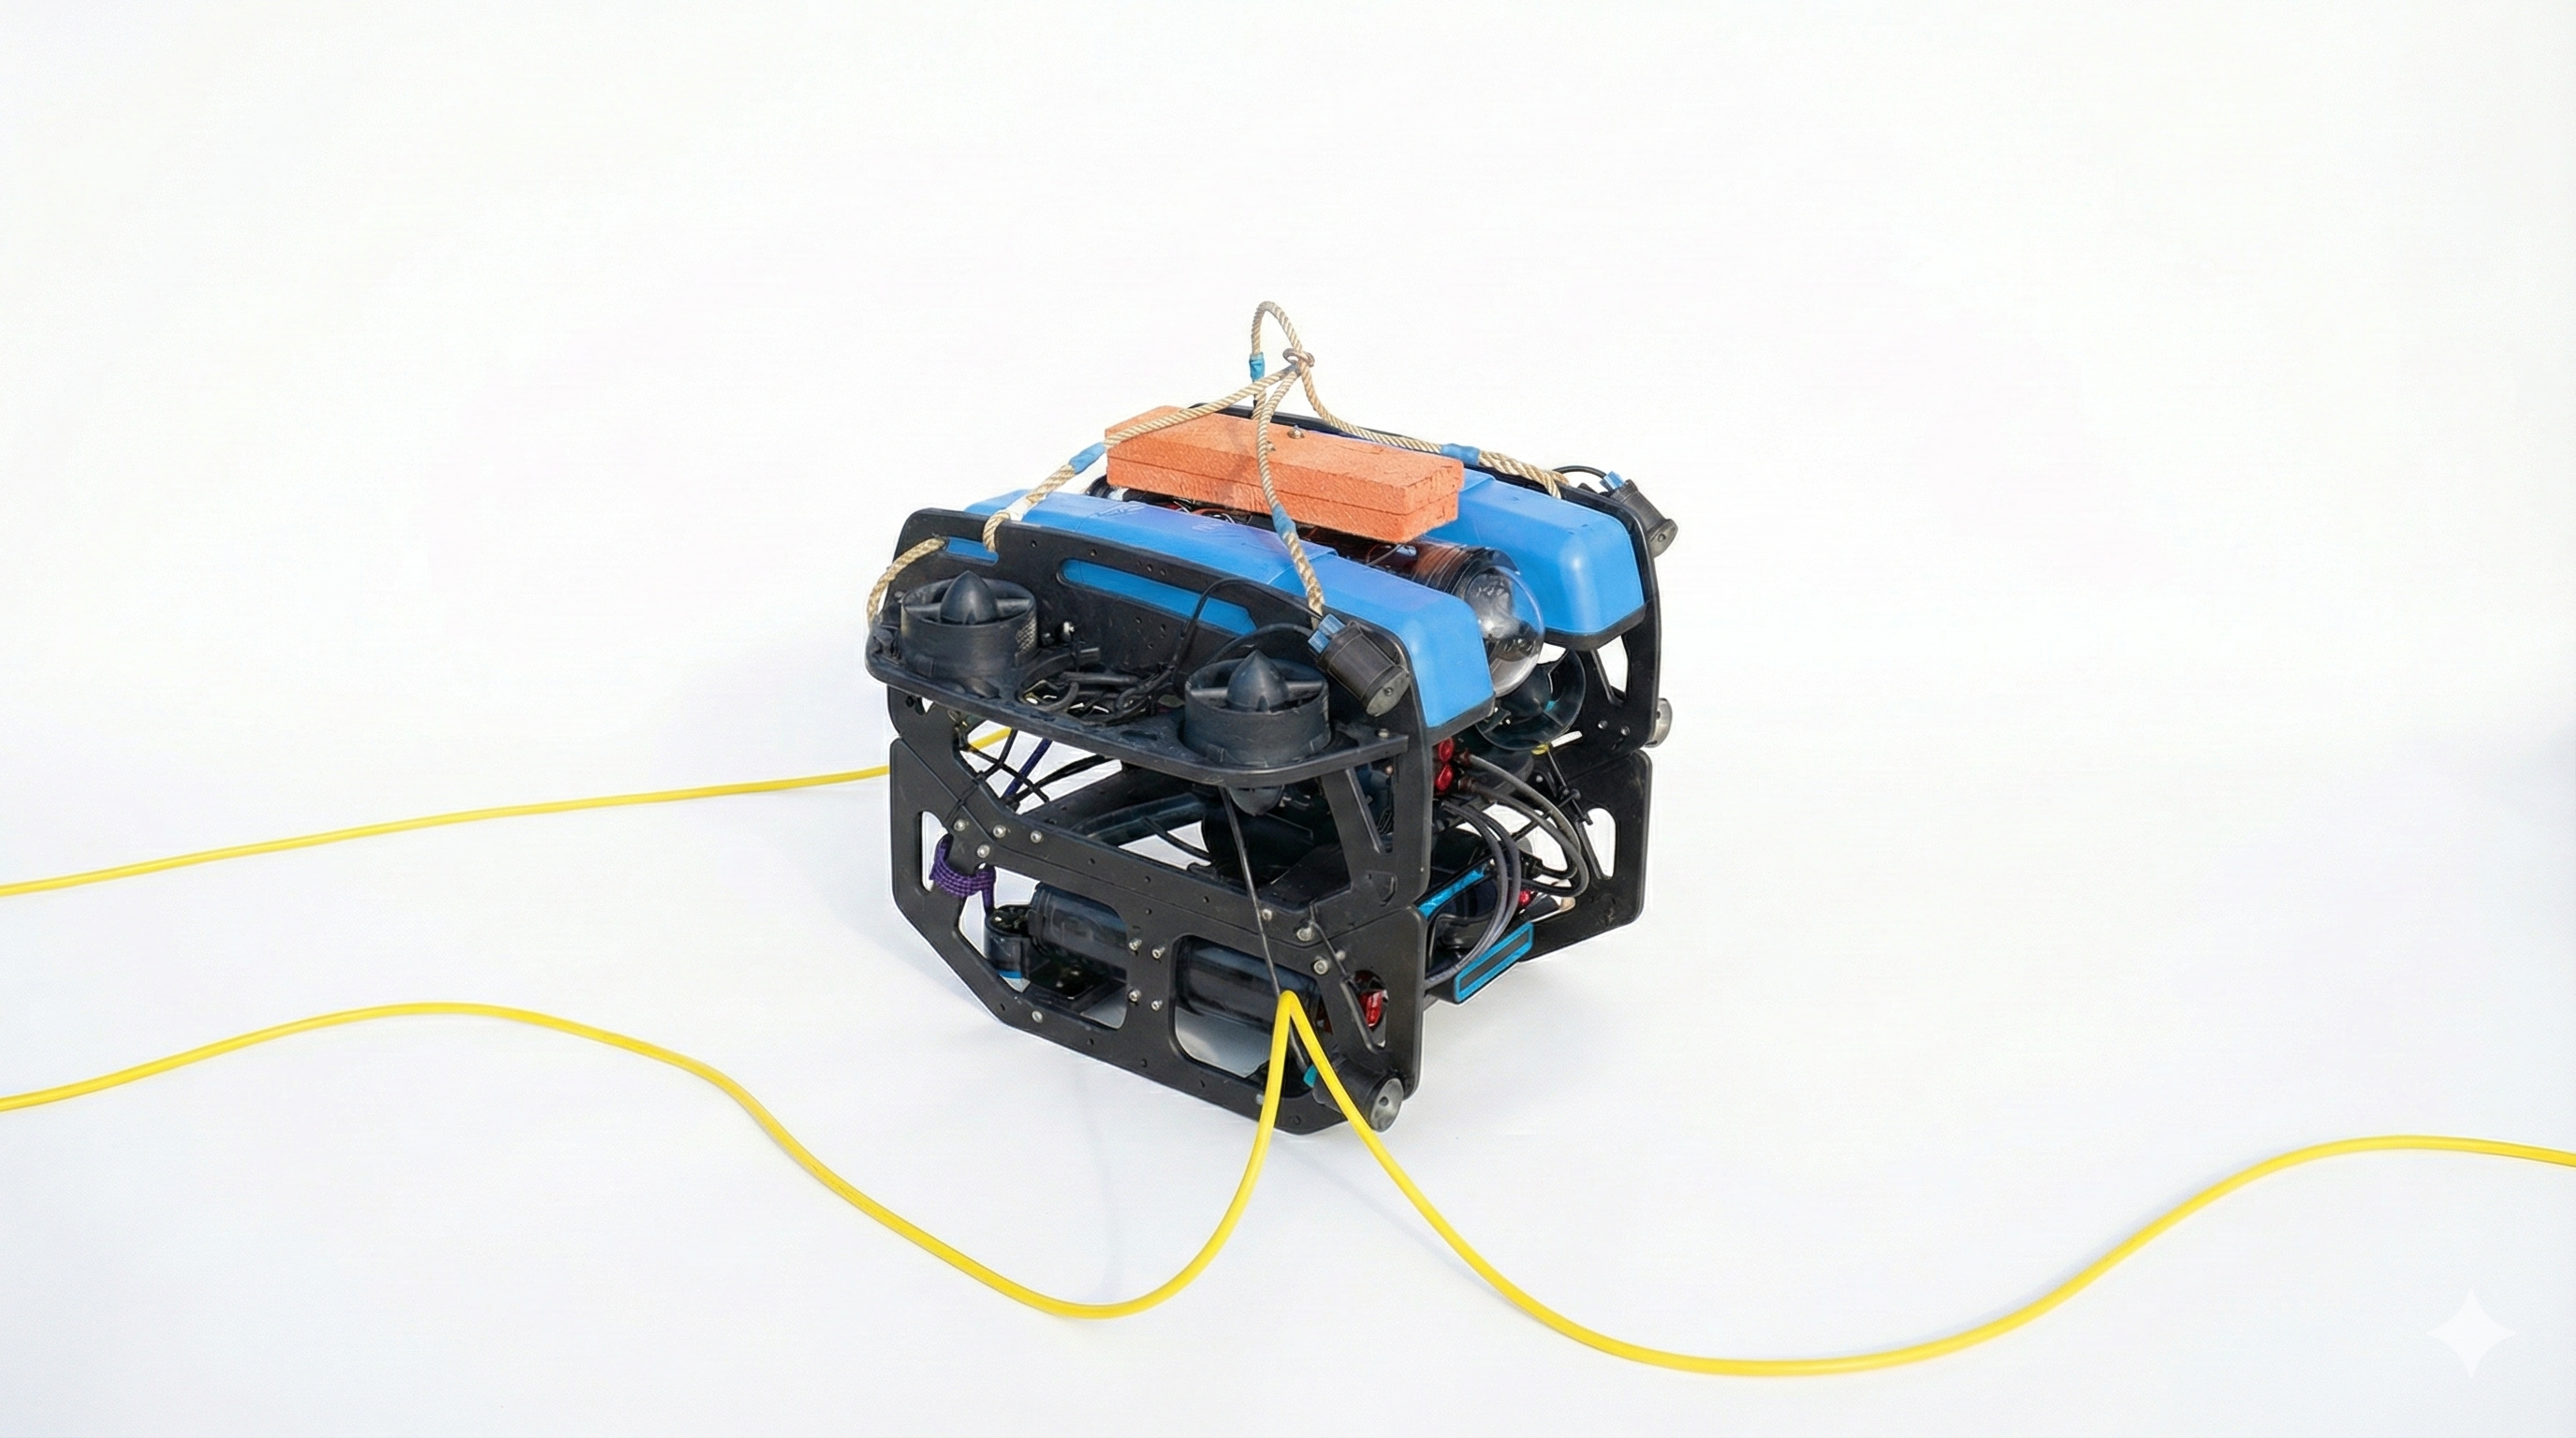
\includegraphics[width=\textwidth]{images/BlueROV.png}
    \caption{Illustration de notre BlueROV}
    \label{fig:bluerov_materiel} % Ensure this label is defined
\end{figure}

La figure \ref{fig:bluerov_materiel} montre notre BlueROV modifié pour le projet de docking autonome.

Pour la perception et le docking, le ROV embarque le sonar multifaisceaux Oculus M750d (Blueprint Subsea). Exploité en haute fréquence (1.2~MHz), il offre la résolution nécessaire aux manœuvres fines : 2.5~mm en portée et $0.6^{\circ}$ en azimut. Il possède une portée allant jusqu'à 120~m. Son ouverture ($130^{\circ}$ horizontal / $20^{\circ}$ vertical) impose un montage incliné vers le bas pour optimiser la visibilité de la cible. L'acquisition des données acoustiques est assurée en temps réel via un driver ROS, permettant leur intégration directe dans la boucle de contrôle autonome.

Nous disposons de deux cordes permettant de remonter le ROV à la surface, ainsi que d'un long câble jaune assurant le contrôle à distance et l'alimentation électrique. Des mousses orange supplémentaires assurent la flottabilité.

L'architecture propulsive du BlueROV Heavy, articulée autour de huit propulseurs (quatre horizontaux et quatre verticaux), confère au véhicule un caractère holonome complet. En effet, cette configuration vectorielle permet de commander indépendamment et simultanément les six degrés de liberté : les trois translations et les trois rotations (lacet, roulis, tangage). L'avantage majeur de cette disposition réside dans sa capacité à offrir une autorité totale sur la stabilisation de l'assiette (roulis et tangage) tout en assurant le maintien en profondeur. Cette omnidirectionnalité garantit une manœuvrabilité fine, permettant au ROV d'effectuer des déplacements latéraux ou verticaux tout en conservant une orientation angulaire fixe — une caractéristique indispensable pour la précision des relevés et la stabilité des interventions en milieu perturbé.

\subsection{Cage et mousses}

Lors de ce projet, nous avons dû concevoir une cage afin de faire amarer le ROV.

Pour commencer, quelques tests ont été réalisés afin de valider le bon fonctionnement de notre algorithme de docking ; nous avons conçu une "porte" simple en PVC, visible sur la figure \ref{fig:cage} :

\begin{figure}[H]
    \centering
    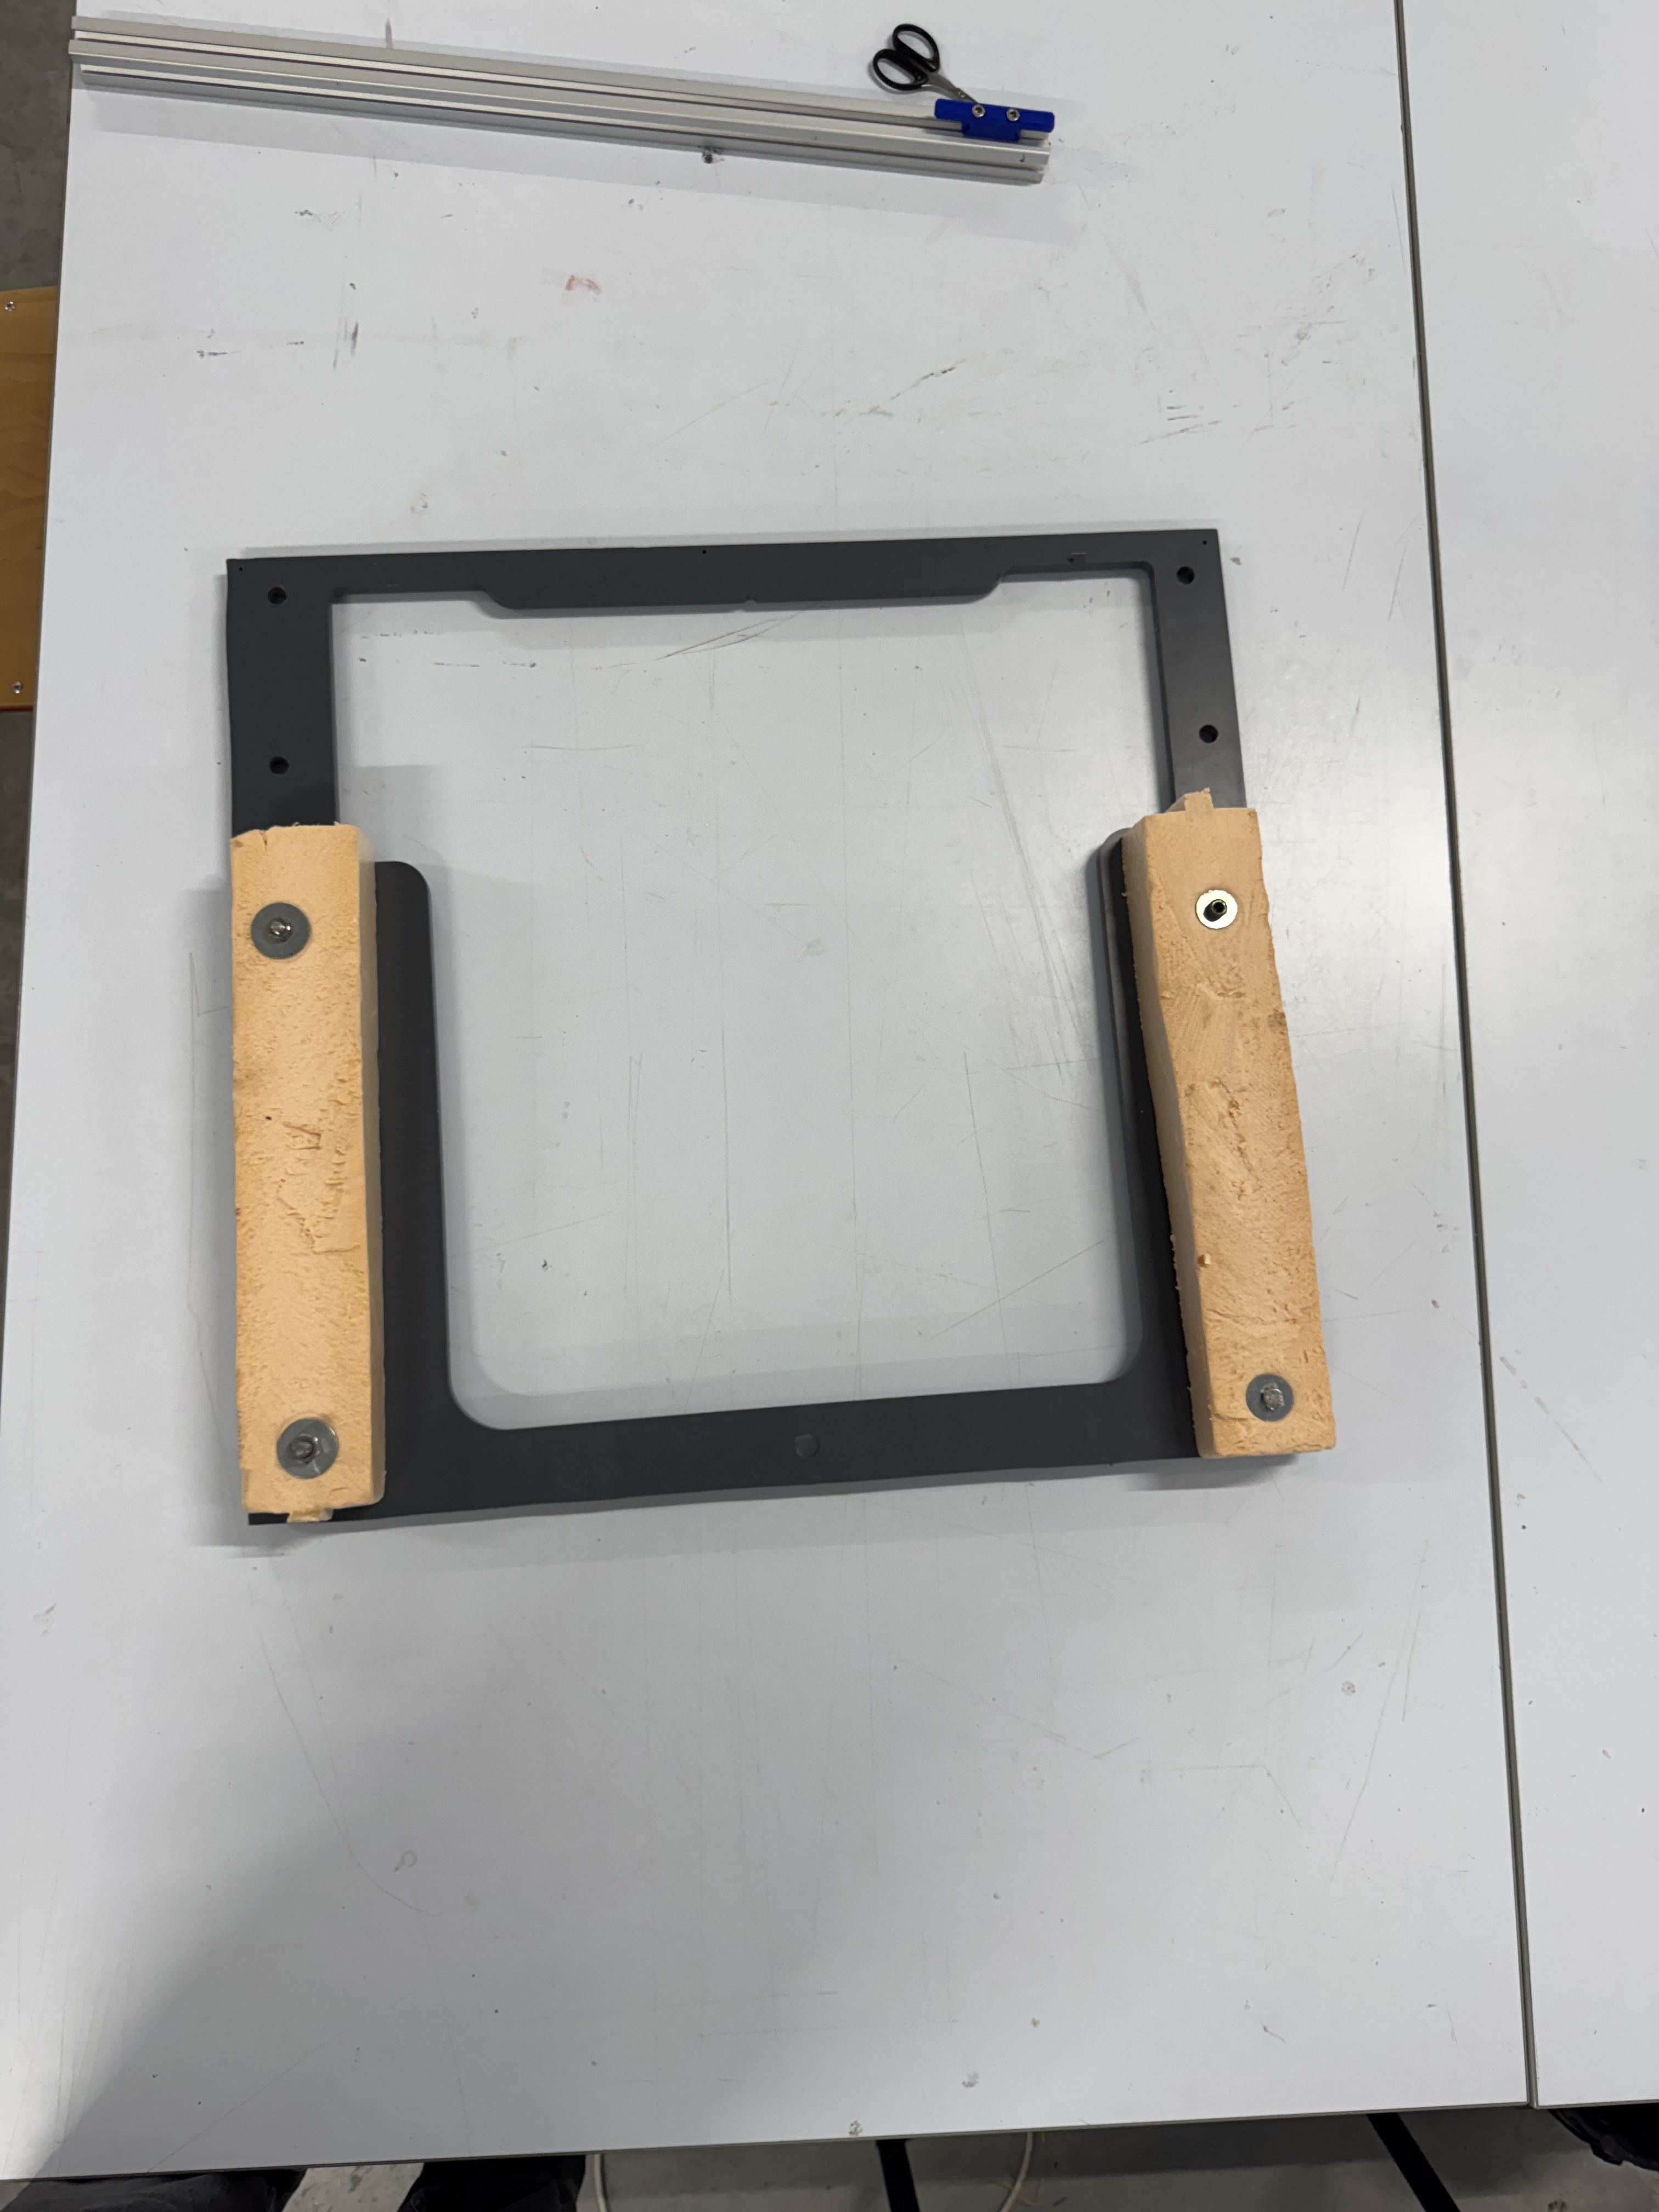
\includegraphics[width=0.6\textwidth]{images/Cage.png}
    \caption{Photographie du premier prototype de cage pour le docking ne représentant qu'une porte}
    \label{fig:cage}
\end{figure}

Afin de la rendre plus visible par ce dernier, nous avons ajouté des pavés de mousses sur les côtés verticaux de la cage.

Nous avons testé plusieurs types de supports permettant de repérer la cage par le sonar. Voici une photo des différents supports testés sur la figure \ref{fig:support_cage} :

\begin{figure}[H]
    \centering
    \includegraphics[width=0.8\textwidth]{images/mousses.jpg}
    \caption{Différents supports testés pour la cage}
    \label{fig:support_cage}
\end{figure}

Voici les résultats des données sonar obtenues lors d'un test en bassin avec la cage équipée des différents supports illustrés sur la figure \ref{fig:support_cage} :



\begin{figure}[H]
    \centering
    % --- Première image ---
    \begin{subfigure}[b]{0.32\textwidth}
        \centering
        \includegraphics[width=\textwidth]{images/mousses_oranges.png}
        \caption{Image sonar avec bouées en mousses}
        \label{fig:mousse_a}
    \end{subfigure}
    % --- Deuxième image ---
    \begin{subfigure}[b]{0.32\textwidth}
        \centering
        \includegraphics[width=\textwidth]{images/parbates.png}
        \caption{Image sonar avec parre-battages}
        \label{fig:mousse_b}
    \end{subfigure}
    % --- Troisième image ---
    \begin{subfigure}[b]{0.32\textwidth}
        \centering
        \includegraphics[width=\textwidth]{images/ptites_bouees_blanches.png}
        \caption{Image sonar avec petites bouées blanches}
        \label{fig:mousse_c}
    \end{subfigure}

    % Légende globale et label global
    \caption{Images sonar des différents supports testés pour la cage}
    \label{fig:supports_cage_tous}
\end{figure}

Le but de la cage est de permettre à l'AUV de se docker. Il faut donc une cage complète (un cube), permettant à l'AUV d'entrer complètement à l'intérieur et d'être maintenu en place lors de manoeuvres de relevage.

Voici une illustration de la cage cubique, en cours de conception, sur la figure \ref{fig:cage_cubique} :

\begin{figure}[H]
    \centering
    \includegraphics[width=0.6\textwidth]{images/cage_cubique.JPEG}
    \caption{Image de notre cage cubique en cours d'assemblage}
    \label{fig:cage_cubique}
\end{figure}

Nous prévoyons d'installer un entonnoir à l'entrée de la cage pour faciliter le docking de l'AUV, le sonar ne nous offrant pas une précision suffisante pour garantir un amarrage parfait sans aide mécanique.

\subsection{Contrôle du robot}

Dans cette partie, nous expliquons la configuration et l'utilisation de la manette. Voici une illustration de celle‑ci, sur la figure \ref{fig:manette} :

\begin{figure}[h!]
    \centering
    \includegraphics[width=0.6\textwidth]{images/manette.png}
    \caption{Image de notre manette}
    \label{fig:manette}
\end{figure}


Pour pouvoir commander le robot via la manette, il faut d'abord l'armer avec la touche « Start ».

Il s'agit d'une sécurité qui permet aussi de désarmer le robot avec la même touche. Si une mission se déroule mal, il est donc possible de désarmer le ROV : aucune commande ne lui sera alors envoyée.

Les lumières sont contrôlées par le bouton « Logitech » au centre de la manette. Initialisées à une valeur PWM de 1000, les lumières sont éteintes. Un appui sur la touche augmente la puissance de 100 jusqu'à la valeur maximale de 2000 ; un nouvel appui la ramène à 1000, éteinte.

Pour pouvoir contrôler les lumières, il faut au moins avoir établi une connexion SSH entre l'ordinateur et le robot une fois, afin d'autoriser les échanges entre le Raspberry Pi (sur lequel sont connectées les lumières) et le code.

Théoriquement, il devrait être possible de commander l'inclinaison de la caméra avec les flèches « haut / bas » à gauche de la manette, mais des problèmes électroniques nous empêchent actuellement d'utiliser cette fonctionnalité.

Concernant le contrôle directionnel, le robot peut se déplacer en translation avec le joystick gauche (L3).

L'orientation (cap) est contrôlée par le joystick droit (R3) de gauche à droite.

La profondeur du robot est commandée par le joystick droit (R3) poussé vers l'avant/arrière : en le poussant vers l'avant, le ROV remonte ; en le poussant vers l'arrière, il descend.

Un régulateur PID a été implémenté pour maintenir une profondeur donnée. Ce mode peut être activé en appuyant sur « X » : lorsqu'on navigue et que le joystick R3 vient d'être relâché, la profondeur actuelle est mémorisée et le PID stabilise le ROV à cette profondeur. Il faut environ une dizaine de secondes pour obtenir une stabilisation quasi‑parfaite, l'action intégrale du PID contribuant à éliminer l'erreur résiduelle.

Un second régulateur PID permet la stabilisation du cap. Il fonctionne de la même façon que l'asservissement de profondeur : lorsque le joystick responsable de l'orientation est relâché, le PID maintient le cap courant.



\subsection{A Faire}

- Préciser l'autonomie de la batterie.

\section{Protocole Expérimental en Bassin}

Une phase préliminaire de conception a été consacrée à la sélection de la géométrie de la cage de docking ainsi qu’au choix des matériaux constitutifs, dans l’objectif de maximiser sa signature acoustique tout en garantissant une intégration mécanique simple. À cette fin, une série de tests exploratoires a été menée en bassin à l’ENSTA. Une cage instrumentée, fixée au centre du bassin, a permis d’évaluer différentes configurations géométriques et solutions matérielles, notamment en termes de réflectivité acoustique et de lisibilité sonar, avant la validation de la configuration retenue pour les essais ultérieurs.

\begin{figure}[h!]
    \centering
    \includegraphics[width=0.6\textwidth]{images/cage_mousse.JPEG}
    \caption{Photographie de la cage instrumentée en bassin}
    \label{fig:cage_bassin}
\end{figure}

\textit{[Instruction : Décrivez les dimensions du bassin (longueur, largeur, profondeur). Expliquez la mise en place de la cage (fixée au fond ou suspendue). Détaillez le scénario de test : position de départ du ROV, procédure de lancement de l'autonomie, critères de succès (entrée complète dans la cage). Mentionnez les outils de vérité terrain utilisés si disponibles (ex: caméras externes pour filmer l'essai).]}

\section{Campagne d'Essais : Lac de Guerlédan}

Afin de valider la robustesse du système en conditions réelles, une campagne a été menée au lac de Guerlédan.

\textit{[Instruction : Décrivez les conditions environnementales spécifiques : turbidité de l'eau (visibilité réduite), présence potentielle de courants, profondeur d'opération. Expliquez les défis logistiques (mise à l'eau depuis un ponton ou un bateau). Comparez la signature acoustique de la cage dans cet environnement "bruité" par rapport au bassin (réverbération du fond, objets parasites).]}

\section{Analyse des Résultats Expérimentaux}

Cette section synthétise les données collectées lors des deux campagnes d'essais.

\textit{[Instruction : Comparez les trajectoires réelles du ROV avec celles de la simulation. Présentez des statistiques de réussite (ex: "Sur 20 tentatives, 15 ont abouti à un amarrage réussi"). Analysez les échecs : est-ce un problème de perte de la cible au sonar (perception) ou une incapacité des propulseurs à contrer une perturbation (commande) ? Incluez des images sonar réelles montrant la cage vue par le robot à différentes distances.]}




